
\chapter{Introduction}
Making an autonomous robot have been the goal of scientists and engineers for years. This
is a difficult task which include many disciplines, and has up to date, not been solved in
a general way. Robots which can reason and take own decisions based on how it senses the
environment would greatly simplify our lives in many ways. Many tasks could be completely
outsourced to autonomous robots which does not tier, and is expendable. This means that it
can go places that a human could not. In short this can be summarized into the three Ds,
namely \emph{dull, dirty} and \emph{dangerous} work. Imagine an autonomous robot going
into a earthquake area and mapping out dangerous spots, and where injured people are,
before medical personnel enter the area. Or a robot mapping and inspecting the vast sewer
network of large city, searching for weak spots and clogged pipes which obstructs the
sewer flow. Or robots crawling the pipelines carrying water, oil or gas to detect leaks
which will cause catastrophic events if not tended to. This are all important work, which
either is dangerous, dirty or dull, or all three at once.

The problem when a robot is going into an unknown area and mapping the surroundings using
a pack of sensors is called \emph{SLAM}, short for Simultaneous Localization and Mapping.
This is a problem much researched around, and have been tried with numerous sensor types
and many algorithms are proposed. Some are best in structured environments, like office
landscapes and industrial areas, while other will preform better in more sparse areas with
less landmarks and recognizable features. 

In our global world the transport of resources, like oil and gas are of great importance. Much of this
transport is done using pipelines. There are millions of kilometers with pipelines around
the world. These pipelines need regular inspections to insure that the pipeline is intact
and undamaged. Also sewers, as mentioned above, needs inspections to keep a satisfactory
standard. Some of the pipes are considered accessible by humans, i.e. diameter over 80 cm,
but most are smaller than this, and uses various inspection devices feeding video to human
operator that must detect, record, and classify the damages. This is tedious work which
can be automated using robots. \cite{MAKRO-project}

One such robot suitable for pipe inspection might be the \emph{Pipe Inspection Konda}
(PIKo) developed by SINTEF. This is a snake like robot, consisting a series of identical
modules interconnected by two degrees of freedom active joints. On each module there is a
set of four wheels, two near the ground and two on on the top of the modules. For
horizontal motion it uses these wheels and a train like motion. Since the joints are
connected with two degrees of freedom, the robot is capable of traversing vertical pipes
as well. This is achieved by spanning the pipe alternately and pushing the wheels towards
the pipe walls to gain enough friction for the robot to motion vertically. \cite{piko}

This report will outline a possible navigation system for PIKo. This include the eyes and
ears, the reasoning needed to interpret the senses, together with recollection of the
areas and the decision making on what to do next. Making the robot do this all by it self
is a tremendous task and has up to date not been solved for the general case.
\begin{figure}[htbp]
    \centering
    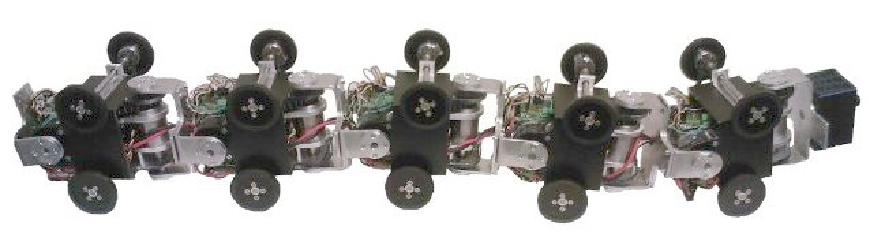
\includegraphics[width=0.8\textwidth]{pics/piko}
    \caption{The Pipe Inspection Konda. \url{www.sintef.no}}
    \label{chap1:fig-piko}
\end{figure}

The challenges with designing such a navigation system is amongst others the difficulties
with keeping track of where the robot is, and more importantly where it has been. This is
difficult in a pipe environment because it does not allow for a redundant positioning
system for global position estimation, such as GPS. The robot is then limited to using
either some kind of odometry or determination and tracking of landmarks in the environment, 
or both. 

When the robot know where it is, it must take the decision on where it is to go, and if
there is something blocking the way, it needs to handle this cases in some way.
Unfortunately, the world is not ideal as the usual lab environments that are used to
verify research. This calls for a robust system which can handle the situations that can
occur in the given mission environments. 

The report will define and select sensors applicable for a pipe inspection mission
preformed by the PIKo robot platform. The benefits and drawbacks of the different sensors
will be assessed in detail. Next, the sensor data must be stored and interpreted in some
way, and important features must be selected. Some of this methods of feature extraction
will be discussed and data set segmentation need to be outlined. 

Given that the robot is autonomous, and the computational abilities and memory available
for the map representation might be limited, this map representation must take this into
account. A map representation with little pre processing takes up much memory, while a
representation which processes the sensor output and estimates features need less space in
memory if the features are recognized by the system. 


\section{Assumptions}
To summarize the points above there are some assumptions which simplifies the problem
treated in this report.
\begin{itemize}
    \item Only planar motion is assumed, even though the implementation platform is
    capable of vertical motion. 
    \item The environment which the robot will operate are structured. Mainly pipe-like
    environments and confined spaces. 
\end{itemize}

\section{Demands}
The complete navigation system for a pipe inspection robot should meet the following
demands and qualities. 
\begin{itemize}
    \item Robustness. The system should be robust and able to take the right decisions
    even when the sensors does not give good readings, at least for a limited time.
    \item Real-time system with limited computational abilities. The system is embedded
    and the processor power and memory available are limited. The algorithms should be
    efficient and the sensor data should be treated and stored in an memory efficient way. 
    \item Simplicity. Make thing as simple as possible but not simpler, a great scientist
    once said. This might help to keep the complexity of the system down. 
    \item Consistency. If the system is presented with the same conditions as the
    decision taken should be consistent.  
\end{itemize}


\section{Structure of the Report}
The report is presented in the following way. Chapter \ref{chap2} give a thorough
introduction to the concepts needed to understand this report. It will address different
range finding techniques, and different sensor concepts will be introduced with advantages
and disadvantages of the concepts. Stereo imaging will be discussed in detail, from camera
calibration, and epipolar geometry to rectification of the captured images and
reprojection of the extracted disparity images. The most used map data representations will be
introduced and explained, also feature extraction and model fitting in Section
\ref{chap2:sec-representations} and \ref{chap2:sec-feature-extraction}. At last a survey
of the different pipe inspection robots currently under research is included in Section
\ref{chap2:sec-state-of-the-art}.

Chapter \ref{chap3} concerns the selection of sensors appropriate for the application, and
calibration of the sensors. The lens distortion parameters and intrinsic parameters of the
sensors will be estimated for the calibration. 

The representation of the world will be treated in Chapter \ref{chap5}. How the sensor
output are interpreted will also be shown in this chapter.

Chapter \ref{chap6} and \ref{chap7} will deal with implementation and testing of the
proposed system. While Chapter \ref{chap8} will discuss how the proposed system preformed
on the tests. The last chapter will give the main conclusions and propose further topics
for research. 
